\documentclass{article}
\usepackage{tikz}
\usepackage{tikz-network}

\begin{document}


\begin{tikzpicture}
\filldraw (-.2,.2) circle (2pt) (.2,.2) circle (2pt);
\draw (0,0) circle (5mm) (-.3,-.1) .. controls (0,-.3) ..
(.3,-.1);
\end{tikzpicture}


\begin{tikzpicture}
\draw (0,0) .. controls (1,1) and (2,1) .. (2,0);
\end{tikzpicture}




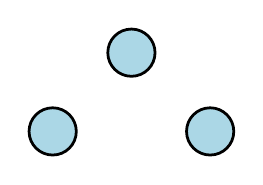
\begin{tikzpicture}
\Vertex{A}
\Vertex[x=1,y=1]{B}
\Vertex[x=2]{C}
\end{tikzpicture}



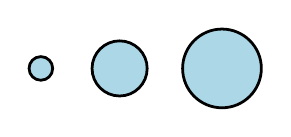
\begin{tikzpicture}
\Vertex[size=.3]{A}
\Vertex[x=1,size=.7]{B}
\Vertex[x=2.3,size=1]{C}
\end{tikzpicture}



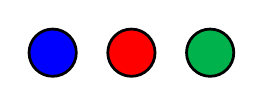
\begin{tikzpicture}
\Vertex[color = blue]{A}
\Vertex[x=1,color=red]{B}
\Vertex[x=2,color=green!70!blue]{C}
\end{tikzpicture}




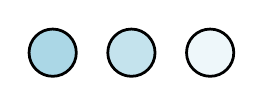
\begin{tikzpicture}
\Vertex[opacity = 1]{A}
\Vertex[x=1,opacity =.7]{B}
\Vertex[x=2,opacity =.2]{C}
\end{tikzpicture}




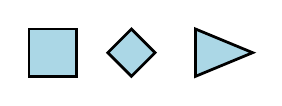
\begin{tikzpicture}
\Vertex[shape = rectangle]{A}
\Vertex[x=1,shape = diamond]{B}
\Vertex[x=2,shape = isosceles triangle]{C}
\end{tikzpicture}



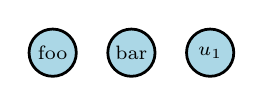
\begin{tikzpicture}
\Vertex[label=foo]{A}
\Vertex[x=1,label=bar]{B}
\Vertex[x=2,label=$u_1$]{C}
\end{tikzpicture}






\begin{tikzpicture}
\Vertex[label=foo,fontsize=\normalsize]{A}
\Vertex[x=1,label=bar,fontsize=\tiny]{B}
\Vertex[x=2,label=$u_1$,fontsize=\large]{C}
\end{tikzpicture}







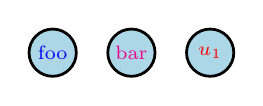
\begin{tikzpicture}
\Vertex[label=foo,fontcolor=blue]{A}
\Vertex[x=1,label=bar,fontcolor=magenta]{B}
\Vertex[x=2,label=$u_1$,fontcolor=red]{C}
\end{tikzpicture}




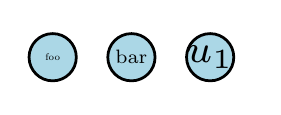
\begin{tikzpicture}
\Vertex[label=foo,fontscale=0.5]{A}
\Vertex[x=1,label=bar,fontscale=1]{B}
\Vertex[x=2,label=$u_1$,fontscale=2]{C}
\end{tikzpicture}




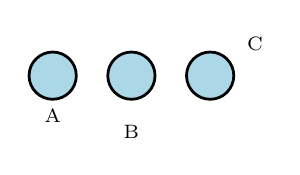
\begin{tikzpicture}
\Vertex[label=A,position=below]{A}
\Vertex[x=1,label=B,position=below,distance=2mm]{B}
\Vertex[x=2,label=C,position=30,distance=1mm]{C}
\end{tikzpicture}





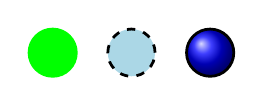
\begin{tikzpicture}
\Vertex[style={color=green}]{A}
\Vertex[x=1,style=dashed]{B}
\Vertex[x=2,style={shading=ball}]{C}
\end{tikzpicture}




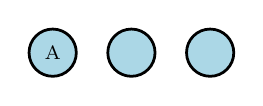
\begin{tikzpicture}
\Vertex[IdAsLabel]{A}
\Vertex[x=1,label=B,NoLabel]{B}
\Vertex[x=2,IdAsLabel,NoLabel]{C}
\end{tikzpicture}





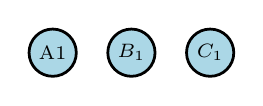
\begin{tikzpicture}
\Vertex[IdAsLabel]{A1}
\Vertex[x=1,label=B_1,Math]{B}
\Vertex[x=2,Math,IdAsLabel]{C_1}
\end{tikzpicture}






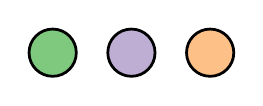
\begin{tikzpicture}
\Vertex[RGB,color={127,201,127}]{A}
\Vertex[x=1,RGB,color={190,174,212}]{B}
\Vertex[x=2,RGB,color={253,192,134}]{C}
\end{tikzpicture}






\begin{tikzpicture}
\Vertex{A}
\Vertex[x=2,Pseudo]{B}
\end{tikzpicture}






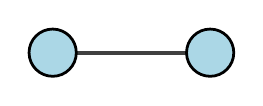
\begin{tikzpicture}
\Vertex{A} \Vertex[x=2]{B}
\Edge(A)(B)
\end{tikzpicture}







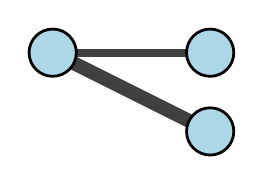
\begin{tikzpicture}
\Vertex{A} \Vertex[x=2]{B} \Vertex[x=2,y=-1]{C}
\Edge[lw=3pt](A)(B)
\Edge[lw=5pt](A)(C)
\end{tikzpicture}






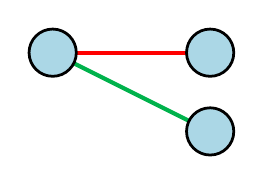
\begin{tikzpicture}
\Vertex{A} \Vertex[x=2]{B} \Vertex[x=2,y=-1]{C}
\Edge[color=red](A)(B)
\Edge[color=green!70!blue](A)(C)
\end{tikzpicture}







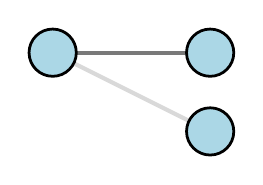
\begin{tikzpicture}
\Vertex{A} \Vertex[x=2]{B} \Vertex[x=2,y=-1]{C}
\Edge[opacity=.7](A)(B)
\Edge[opacity=.2](A)(C)
\end{tikzpicture}






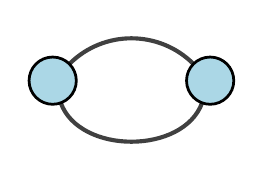
\begin{tikzpicture}
\Vertex{A} \Vertex[x=2]{B}
\Edge[bend=45](A)(B)
\Edge[bend=-70](A)(B)
\end{tikzpicture}







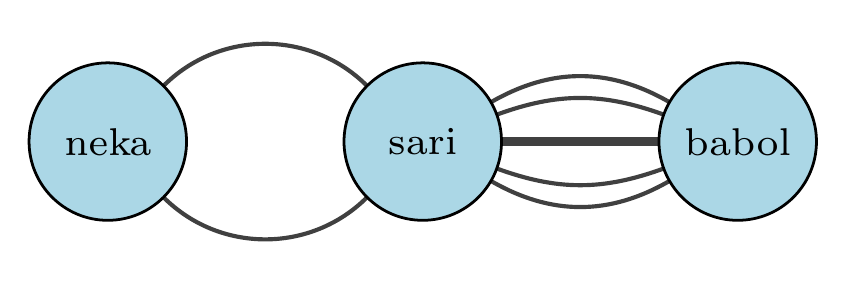
\begin{tikzpicture}
\Vertex[x=0,label=neka,size=2,fontscale=2]{A} 
\Vertex[x=4,label=sari,size=2,fontscale=2]{B}
\Vertex[x=8,label=babol,size=2,fontscale=2]{C}

\Edge[bend=45](A)(B)
\Edge[bend=-45](A)(B)

\Edge[bend=30](B)(C)
\Edge[bend=20](B)(C)
\Edge[bend=0,lw=3pt](B)(C)
\Edge[bend=-20](B)(C)
\Edge[bend=-30](B)(C)

\end{tikzpicture}





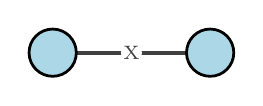
\begin{tikzpicture}
\Vertex{A} \Vertex[x=2]{B}
\Edge[label=X](A)(B)
\end{tikzpicture}






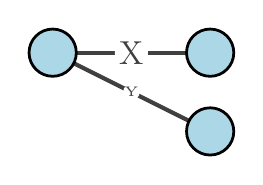
\begin{tikzpicture}
\Vertex{A} \Vertex[x=2]{B} \Vertex[x=2,y=-1]{C}
\Edge[label=X,fontsize=\large](A)(B)
\Edge[label=Y,fontsize=\tiny](A)(C)
\end{tikzpicture}





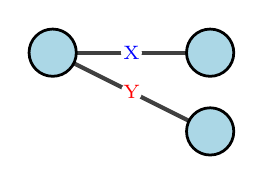
\begin{tikzpicture}
\Vertex{A} \Vertex[x=2]{B} \Vertex[x=2,y=-1]{C}
\Edge[label=X,fontcolor=blue](A)(B)
\Edge[label=Y,fontcolor=red](A)(C)
\end{tikzpicture}






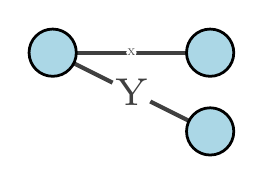
\begin{tikzpicture}
\Vertex{A} \Vertex[x=2]{B} \Vertex[x=2,y=-1]{C}
\Edge[label=X,fontscale=.5](A)(B)
\Edge[label=Y,fontscale=2](A)(C)
\end{tikzpicture}






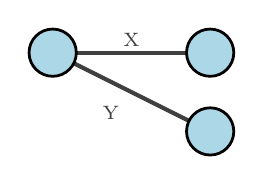
\begin{tikzpicture}
\Vertex{A} \Vertex[x=2]{B} \Vertex[x=2,y=-1]{C}
\Edge[label=X,position=above](A)(B)
\Edge[label=Y,position={below left=2mm}](A)(C)
\end{tikzpicture}







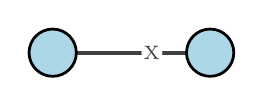
\begin{tikzpicture}
\Vertex{A} \Vertex[x=2]{B}
\Edge[label=X,distance=.7](A)(B)
\end{tikzpicture}






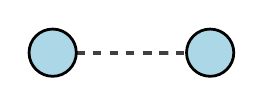
\begin{tikzpicture}
\Vertex{A} \Vertex[x=2]{B}
\Edge[style={dashed}](A)(B)
\end{tikzpicture}






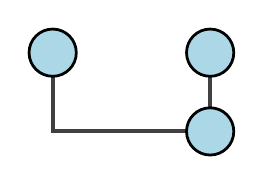
\begin{tikzpicture}
\Vertex{A} \Vertex[x=2]{B} \Vertex[x=2,y=-1]{C}
\Edge[path={A,{0,-1},C,B}](A)(B)
\end{tikzpicture}





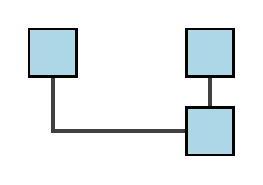
\begin{tikzpicture}
\Vertex[shape = rectangle]{A} 
\Vertex[x=2,shape = rectangle]{B} 
\Vertex[x=2,y=-1,shape = rectangle]{C}
\Edge[path={A,{0,-1},C,B}](A)(B)
\end{tikzpicture}








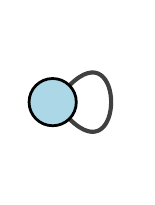
\begin{tikzpicture}
\Vertex{A}
\Edge(A)(A)
\end{tikzpicture}








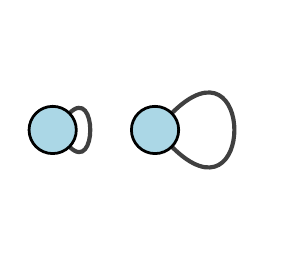
\begin{tikzpicture}
\Vertex{A} \Vertex[x=1.3]{B}
\Edge[loopsize=.5cm](A)(A)
\Edge[loopsize=1.5cm](B)(B)
\end{tikzpicture}








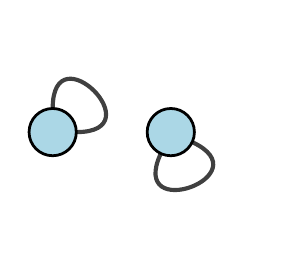
\begin{tikzpicture}
\Vertex{A} \Vertex[x=1.5]{B}
\Edge[loopposition=45](A)(A)
\Edge[loopposition=-70](B)(B)
\end{tikzpicture}









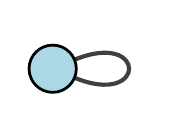
\begin{tikzpicture}
\Vertex{A}
\Edge[loopshape=45](A)(A)
\end{tikzpicture}








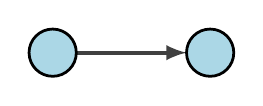
\begin{tikzpicture}
\Vertex{A} \Vertex[x=2]{B}
\Edge[Direct](A)(B)
\end{tikzpicture}









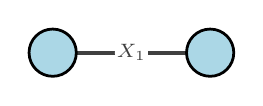
\begin{tikzpicture}
\Vertex{A} \Vertex[x=2]{B}
\Edge[Math,label=X_1](A)(B)
\end{tikzpicture}







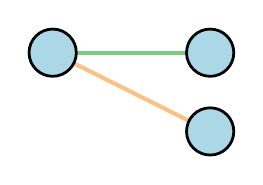
\begin{tikzpicture}
\Vertex{A} \Vertex[x=2]{B} \Vertex[x=2,y=-1]{C}
\Edge[RGB,color={127,201,127}](A)(B)
\Edge[RGB,color={253,192,134}](A)(C)
\end{tikzpicture}








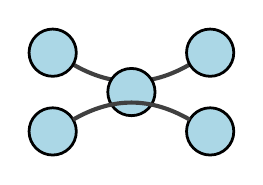
\begin{tikzpicture}
\Vertex{A} \Vertex[x=2]{B} \Vertex[x=1,y=-.5]{C}
\Vertex[y=-1]{D} \Vertex[x=2,y=-1]{E}
\Edge[bend=-30](A)(B)
\Edge[bend=30,NotInBG](D)(E)
\end{tikzpicture}






\begin{tikzpicture}
\Text{A}
\Text[x=1,y=1]{B}
\Text[x=2]{C}
\end{tikzpicture}








\begin{tikzpicture}
\Text[fontsize=\small]{A}
\Text[x=1,fontsize=\LARGE]{B}
\Text[x=2,fontsize=\Huge]{C}
\end{tikzpicture}









\begin{tikzpicture}
\Text[color = blue]{A}
\Text[x=1,color=red]{B}
\Text[x=2,color=green!70!blue]{C}
\end{tikzpicture}










\begin{tikzpicture}
\Text[opacity = 1]{A}
\Text[x=1,opacity =.7]{B}
\Text[x=2,opacity =.2]{C}
\end{tikzpicture}







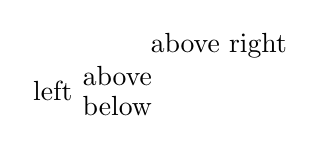
\begin{tikzpicture}
\Text[position=above]{above}
\Text[position=below]{below}
\Text[position=left,distance=5mm]{left}
\Text[position=above right,distance=5mm]{above right}
\end{tikzpicture}






\begin{tikzpicture}
\Text[rotation=30]{A}
\Text[x=1,rotation=45]{B}
\Text[x=2,rotation=75]{C}
\end{tikzpicture}







\begin{tikzpicture}
\Text[anchor=north east]{NE}
\Text[x=1,anchor = south]{S}
\Text[x=2,anchor =south west]{SW}
\end{tikzpicture}







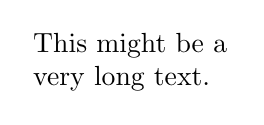
\begin{tikzpicture}
\Text[width=2.5cm]{This might be a very long text.}
\end{tikzpicture}








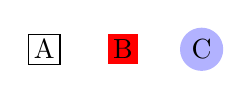
\begin{tikzpicture}
\Text[style={draw,rectangle}]{A}
\Text[x=1,style={fill=red}]{B}
\Text[x=2,style={fill=blue,circle,opacity=.3}]{C}
\end{tikzpicture}








\begin{tikzpicture}
\Text[RGB,color={127,201,127}]{A}
\Text[x=1,RGB,color={190,174,212}]{B}
\Text[x=2,RGB,color={253,192,134}]{C}
\end{tikzpicture}














\end{document}